\documentclass[12pt, titlepage]{article}

\usepackage{booktabs}
\usepackage{tabularx}
\usepackage{hyperref}
\hypersetup{
    colorlinks,
    citecolor=black,
    filecolor=black,
    linkcolor=red,
    urlcolor=blue
}
\usepackage[round]{natbib}
\usepackage{graphicx}
\usepackage{subfig}

%% Comments

\usepackage{color}

\newif\ifcomments\commentstrue %displays comments
%\newif\ifcomments\commentsfalse %so that comments do not display

\ifcomments
\newcommand{\authornote}[3]{\textcolor{#1}{[#3 ---#2]}}
\newcommand{\todo}[1]{\textcolor{red}{[TODO: #1]}}
\else
\newcommand{\authornote}[3]{}
\newcommand{\todo}[1]{}
\fi

\newcommand{\wss}[1]{\authornote{blue}{SS}{#1}} 
\newcommand{\plt}[1]{\authornote{magenta}{TPLT}{#1}} %For explanation of the template
\newcommand{\an}[1]{\authornote{cyan}{Author}{#1}}

%% Common Parts

\newcommand{\progname}{ProgName} % PUT YOUR PROGRAM NAME HERE
\newcommand{\authname}{Team \#, Team Name
\\ Student 1 name
\\ Student 2 name
\\ Student 3 name
\\ Student 4 name} % AUTHOR NAMES                  

\usepackage{hyperref}
    \hypersetup{colorlinks=true, linkcolor=blue, citecolor=blue, filecolor=blue,
                urlcolor=blue, unicode=false}
    \urlstyle{same}
                                


\begin{document}

\title{Verification and Validation Report: \progname} 
\author{\authname}
\date{\today}
	
\maketitle

\pagenumbering{roman}

\section{Revision History}

\begin{tabularx}{\textwidth}{p{3cm}p{2cm}X}
\toprule {\bf Date} & {\bf Version} & {\bf Notes}\\
\midrule
2025-04-16 & Rev 1.0 & Initial Release\\
\bottomrule
\end{tabularx}

~\newpage

\section{Symbols, Abbreviations and Acronyms}

\renewcommand{\arraystretch}{1.2}
\begin{tabular}{l l} 
  \toprule		
  \textbf{symbol} & \textbf{description}\\
  \midrule 
  CSV & comma separated value \\
  FAST & Features from Accelerated Segment Test \\
  IFCS & \progname{} software\\
  T & Test\\
  \bottomrule
\end{tabular}\\


\newpage

\tableofcontents

\listoftables %if appropriate

\listoffigures %if appropriate

\newpage

\pagenumbering{arabic}

This document outlines the results of the system and unit tests for the \progname  $ $ software. The detaileds of the associated tests are outlined in the \href{https://github.com/KiranSingh15/CAS-741-Image-Correspondences/blob/main/docs/VnVPlan/VnVPlan.pdf}{\textbf{VnV Plan}}.
\section{Functional Requirements Evaluation}


\subsection{Feature Detection}
\paragraph{Image Smoother}

\begin{enumerate}
\item \hypertarget{STFR-IS-01}{\textbf{STFR-IS-01}} \\ \\ 
This test evaluates the capacity of the system to import generated ArUco marker imagery, convert the imagery to a greyscale format, perform Gaussian smoothing, and save both the greyscale and smoothed images using a kernel size of 5 and a standard deviation of 1.0. This test was manually initiated and executed via Pytest using the \href{https://github.com/KiranSingh15/CAS-741-Image-Correspondences/blob/main/src/tests/test_STFR-IS-01.py}{test\_STFR-IS-01.py} program. The test passed all checks and provides a \href{https://github.com/KiranSingh15/CAS-741-Image-Correspondences/blob/main/src/tests/Outputs/2025-04-13_12-19-08/summary.txt}{summary.txt} of the results under its timestamped \href{https://github.com/KiranSingh15/CAS-741-Image-Correspondences/tree/main/src/tests/Outputs/2025-04-13_12-19-08}{STFR-IS-01} output folder. \\ \\
\textit{Requirements Addressed:}
\begin{itemize}
\item R1 (Update Image Noise) 
\item R5 (Default Noise Suppression)
\item R9 (Perform Noise Reduction)
\end{itemize}

Figure \ref{fig-IS-AR} shows an example of the generated greyscale and smoothed imagery of the ArUco markers. All generated output imagery can be reviewed in the \href{https://github.com/KiranSingh15/CAS-741-Image-Correspondences/tree/main/src/tests/Outputs/2025-04-13_12-19-08}{STFR-IS-01} output folder.\\


\begin{figure}[h!]
  \centering
  \subfloat[Converted Greyscale Image \label{AR-GS}]{
  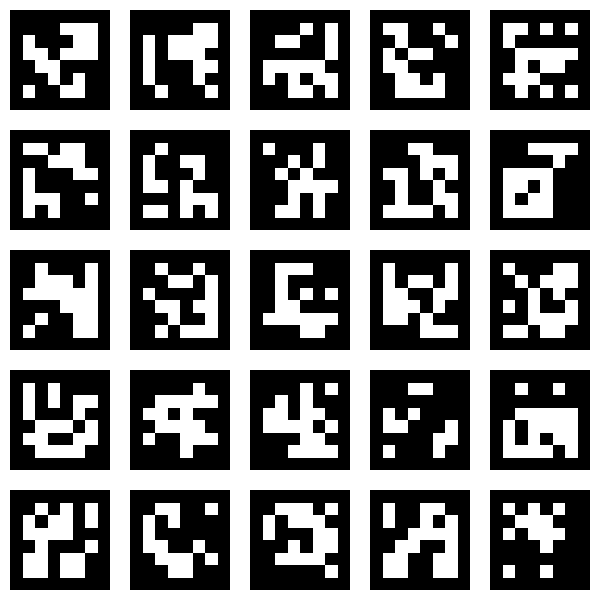
\includegraphics[width=0.45\linewidth]{images/gs_aruco_000.png}
  }
  \hfill
  \subfloat[Gaussian-Smoothed Image \label{AR-GK}]{
  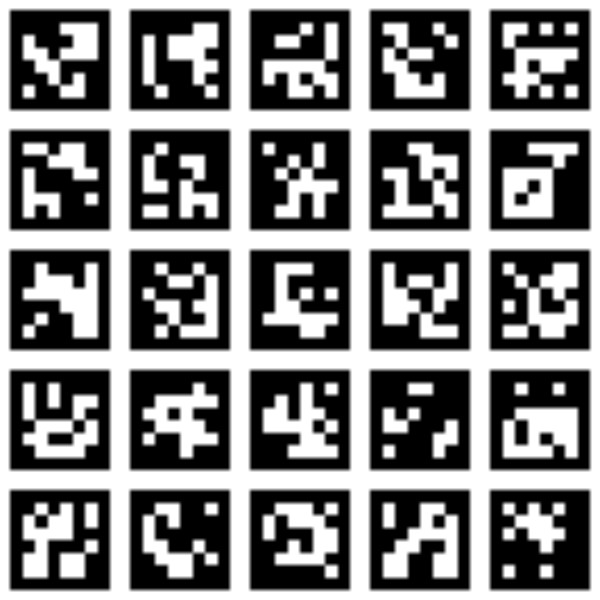
\includegraphics[width=0.45\linewidth]{images/aruco_000.png}
  }
  \caption{Outputs of the image smoothing procedure on an untransformed ArUco marker}
  \label{fig-IS-AR}
\end{figure}


As the results from processing a binary ArUco marker do not produce a distinct change in colour to the human eye, a second test was executed on the test imagery provided in the \href{https://github.com/KiranSingh15/CAS-741-Image-Correspondences/tree/main/src/tests/testImages/building}{testImages\textbackslash building} folder.

\begin{figure}[h!]
  \centering
  \subfloat[Building - RGB Input Image \label{UH-IN}]{
  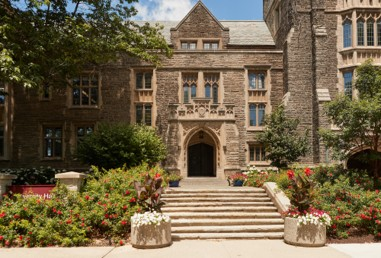
\includegraphics[width=0.45\linewidth]{images/UH_raw.jpg}
  }
  \hfill
  \subfloat[Building - Greyscale Image \label{UH-GS}]{
  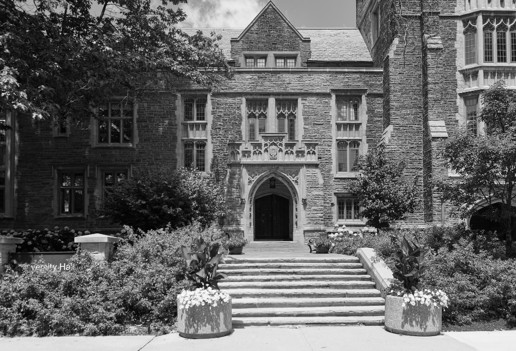
\includegraphics[width=0.45\linewidth]{images/UH_gs.jpg}
  }
  \hfill
  \subfloat[Building - Smoothed Image \label{UH-SM}]{
  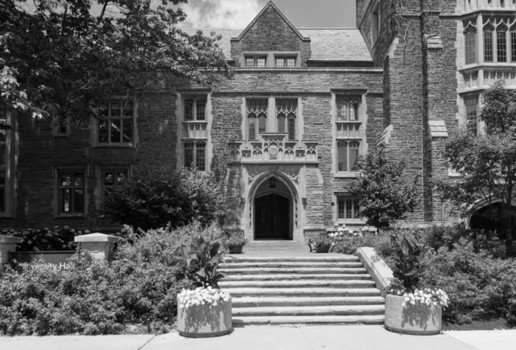
\includegraphics[width=0.45\linewidth]{images/UH_is.jpg}
  }
  \caption{Greyscale and noise-reduced images generated from the building dataset}
  \label{fig-building}
\end{figure}

\end{enumerate}

\newpage

\paragraph{Keypoint Detection}
\begin{enumerate}

\item \hypertarget{STFR-KP-01}{\textbf{STFR-KP-01}}\\
This test evaluates the capacity of the system to import smoothed ArUco marker imagery and identify keypoints through use of rotated-FAST methods. A pixel intensity threshold of 60 was set for this test. This test was manually initiated and executed via Pytest using the \href{https://github.com/KiranSingh15/CAS-741-Image-Correspondences/blob/main/src/tests/test_STFR-KP-01.py}{test\_STFR-KP-01.py} program. The test successfully passed all checks and provides a \href{https://github.com/KiranSingh15/CAS-741-Image-Correspondences/blob/main/src/tests/Outputs/2025-04-13_12-20-06/summary.txt}{summary.txt} of the results under its timestamped \href{https://github.com/KiranSingh15/CAS-741-Image-Correspondences/tree/main/src/tests/Outputs/2025-04-13_12-20-06}{STFR-KP-01} output folder. \\ \\
\textit{Requirements Addressed:} 
\begin{itemize}
\item R2 (Update Pixel Intensity Threshold)
\item R6 (Perform Corner Detection)
\item R10 (Identify Keypoints)
\end{itemize}

Figure \ref{fig-KP-AR} shows an example of the generated greyscale and smoothed imagery of the ArUco markers. All generated output imagery and corresponding CSV files can be reviewed in the \href{https://github.com/KiranSingh15/CAS-741-Image-Correspondences/tree/main/src/tests/Outputs/2025-04-13_12-19-08}{STFR-KP-01} output folder.\\

\begin{figure}[h!]
  \centering
  \subfloat[ArUco\_000 with keypoints \label{AR-KP-01}]{
  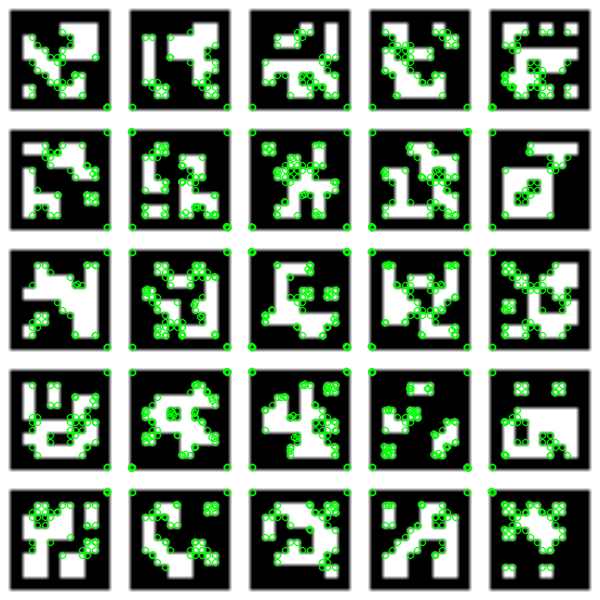
\includegraphics[width=0.45\linewidth]{images/kp_aruco_000.png}
  }
  \hfill
  \subfloat[ArUco\_001 with keypoints \label{AR-KP-02}]{
  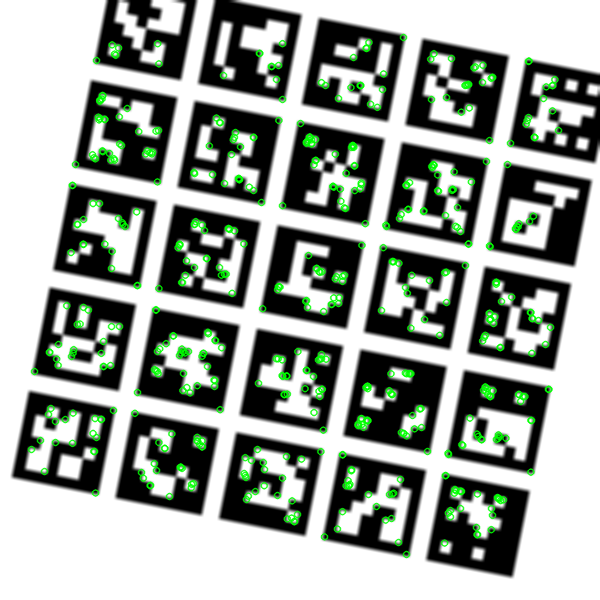
\includegraphics[width=0.45\linewidth]{images/kp_aruco_001.png}
  }
  \caption{Generated images of the keypoint detection test with mapped keypoints}
  \label{fig-KP-AR}
\end{figure}
\end{enumerate}

\paragraph{Feature Description}
\begin{enumerate}
\item \hypertarget{STFR-FD-01}{\textbf{STFR-FD-01}\\}
This test evaluates the capacity of the system to create oriented-BRIEF descriptors using identified keypoints from smoothed greyscale imagery. A target of 100 was set with a search patch size of 31. This test was manually initiated and executed via Pytest using the \href{https://github.com/KiranSingh15/CAS-741-Image-Correspondences/blob/main/src/tests/test_STFR-FD-01.py}{test\_STFR-FD-01.py} program. The test successfully passed all checks and provides a \href{https://github.com/KiranSingh15/CAS-741-Image-Correspondences/blob/main/src/tests/Outputs/2025-04-13_12-17-18/summary.txt}{summary.txt} of the results under its timestamped \href{https://github.com/KiranSingh15/CAS-741-Image-Correspondences/tree/main/src/tests/Outputs/2025-04-13_12-17-18}{STFR-FD-01} output folder. \\ \\
\textit{Requirements Addressed:} 
\begin{itemize}
\item R3 (Update Patch Size)
\item R4 (Update Descriptor Bin Size)
\item R7 (Binary Descriptors)
\item R11 (Define Descriptors)
\end{itemize}

Figure \ref{fig-FD-AR} shows an example of two ArUco markers with keypoints scaled per their feature descriptors. All generated output imagery and corresponding CSV files can be reviewed in the \href{https://github.com/KiranSingh15/CAS-741-Image-Correspondences/tree/main/src/tests/Outputs/2025-04-13_12-17-18}{STFR-FD-01} output folder.\\


\begin{figure}[h!]
  \centering
  \subfloat[ArUco\_000 with scaled keypoints \label{AR-FD-01}]{
  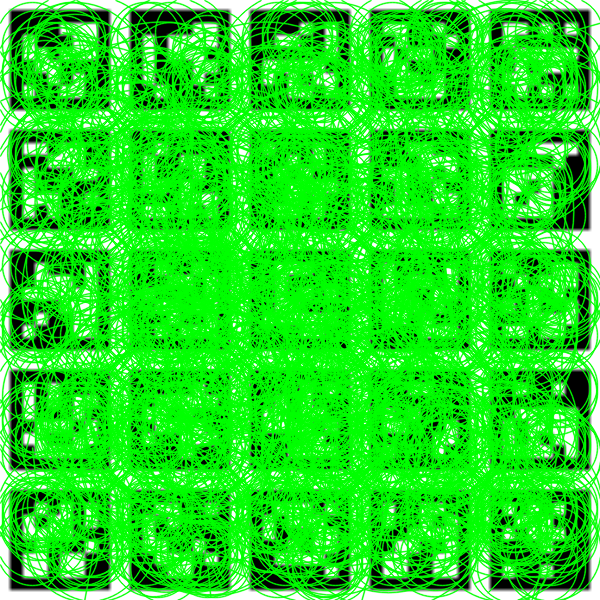
\includegraphics[width=0.45\linewidth]{images/fd_aruco_000.png}
  }
  \hfill
  \subfloat[ArUco\_001 with scaled keypoints \label{AR-FD-02}]{
  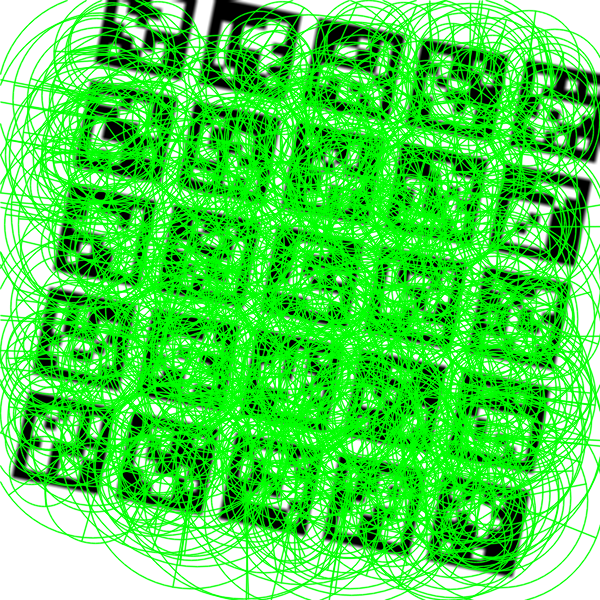
\includegraphics[width=0.45\linewidth]{images/fd_aruco_001.png}
  }
  \caption{Generated images of the keypoint detection test with mapped keypoints}
  \label{fig-FD-AR}
\end{figure}
\end{enumerate}




\subsection{Feature Comparison}
\paragraph{Descriptor Comparison} 

\begin{enumerate}


\item \hypertarget{STFR-FM-01}{\textbf{STFR-FM-01}}\\
This test evaluates the capacity of the system to compare two sets of predefined feature descriptor between two similar images. Using brute-force matching, a maximum Hamming distance of 25 was set for displayed images. Additionally, a maximum of 30 match candidates were permitted to be displayed in the generated imagery. This test was manually initiated and executed via Pytest using the \href{https://github.com/KiranSingh15/CAS-741-Image-Correspondences/blob/main/src/tests/test_STFR-FM-01.py}{test\_STFR-FM-01.py} program. The test successfully passed all checks and provides a \href{https://github.com/KiranSingh15/CAS-741-Image-Correspondences/blob/main/src/tests/Outputs/2025-04-13_12-18-08/summary.txt}{summary.txt} of the results under its timestamped \href{https://github.com/KiranSingh15/CAS-741-Image-Correspondences/tree/main/src/tests/Outputs/2025-04-13_12-18-08}{STFR-FM-01} output folder. \\ \\
\textit{Requirements Addressed:} 
\begin{itemize}
\item R8 (Descriptor Comparison - Hamming Distance)
\item R12 (Search for Matches Candidates)
\item R13 (Verify Match Candidates)
\item R14 (Confirm Pose Identifiers)
\item R15 (Report Match Candidates)
\end{itemize}

Figure \ref{fig-FM-AR} shows an example of thirty candidate feature matches between markers ArUco\_000 and ArUco\_001. All generated output imagery and corresponding CSV files can be reviewed in the \href{https://github.com/KiranSingh15/CAS-741-Image-Correspondences/tree/main/src/tests/Outputs/2025-04-13_12-18-08}{STFR-FM-01} output folder.\\

\begin{figure}
  \centering
  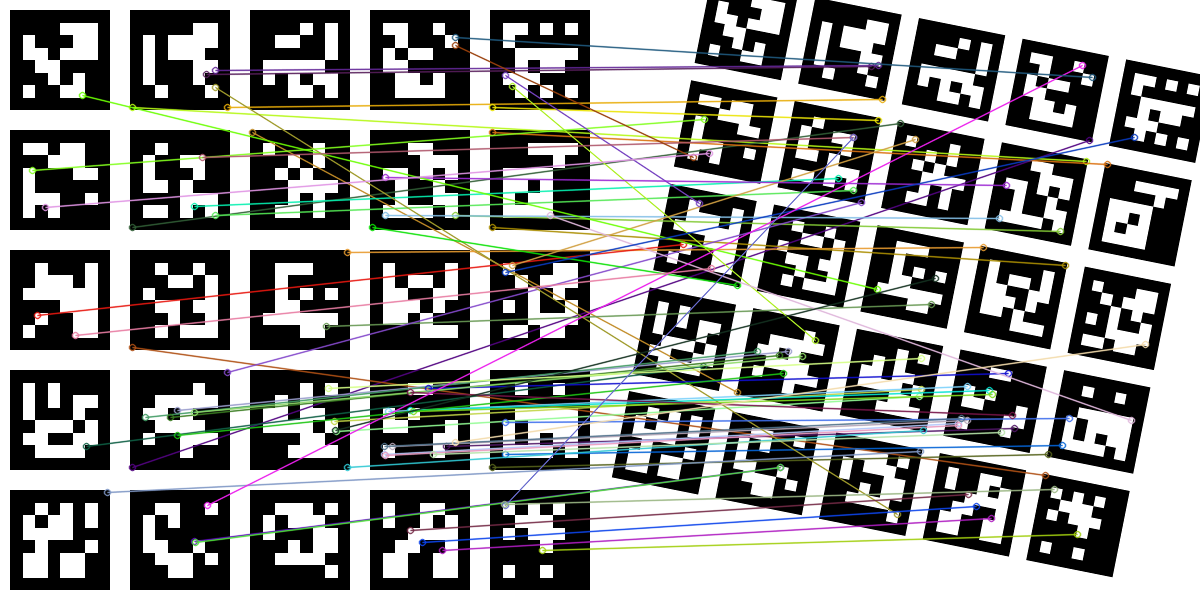
\includegraphics[width=0.95\linewidth]{images/aruco_000_aruco_001.png}
  \caption{Optimal candidate matches between ArUco\_000 and ArUco\_001}
  \label{fig-FM-AR}
\end{figure}



\end{enumerate}



\section{Nonfunctional Requirements Evaluation}
\subsection{Reliability}
\begin{itemize}
  \item NFR1 (Invariance to the Order of Images)
  \end{itemize}
A test script named \href{https://github.com/KiranSingh15/CAS-741-Image-Correspondences/blob/main/src/tests/test_STNFR-RE-01.py}{\textbf{test\_STNFR-RE-01.py}} was prepared. In this script, two images from the \href{https://github.com/KiranSingh15/CAS-741-Image-Correspondences/tree/main/src/tests/testImages/lego}{\textbf{Lego}} image set are renamed and reordered, as outlined in the \href{https://github.com/KiranSingh15/CAS-741-Image-Correspondences/tree/main/src/tests/testImages/lego_swap}{\textbf{Lego\_Swap}} folder. Both of these datasets are processed to identify candidate matches. The resulting match candidates are compared between each data set to confirm that each descriptor and corresponding coordinates from the Lego dataset is matched to the equivalent descriptor in the transformed Lego\_Swap dataset. This test passed with zero errors, and the results are summarized in the \href{https://github.com/KiranSingh15/CAS-741-Image-Correspondences/tree/main/src/tests/Outputs/2025-04-13_15-19-26}{\textbf{STNFR-RE-01}}.


\subsection{Usability}
Ten (10) individuals were given a demonstration of the IFCS software, which included a detailed walkthough of the download process, installation processes, and setup of the virtual environment. Audience members were shown how to add new images from the provided library to the inputs folder, adjust the methods and parameters of image processing, and initiate the IFCS pipeline. Once completed, audience members were shown the following outputs.
\begin{itemize}
  \item generated greyscale imagery
  \item generated smoothed imagery
  \item generated imagery with keypoints
  \item generated imagery with descriptors
  \item generated imagery that compare images with candidate descriptor matches
  \item CSV files of keypoints, descriptors and candidate matches
\end{itemize}
Following the demonstration, a show-of-hands identified that seven (7) of ten audience members stated that they have a favourable opinion of the software and its simplicity of use. At a success rate of 70\%, this fall below the target rate of 80\%. However, this may be improved with the implementation of any one of a user manual, user walkthrough video, or a one-on-one training session with one of the IFCS developers.

\subsection{Maintainability}
\textit{Requirements Addressed:} 
\begin{itemize}
\item NFR3 (Allocation of Developer Resources for New Features)
\end{itemize}
Per the \href{https://github.com/KiranSingh15/CAS-741-Image-Correspondences/blob/main/docs/VnVPlan/VnVPlan.pdf}{\textbf{VnV Plan}}, this requirement has been identified as out of scope for the Rev 1.0 release.
		
\subsection{Performance}
\textit{Requirements Addressed:} 
\begin{itemize}
\item NFR4 (Timing Metrics)
\item NFR5 (Memory Usage Metrics)
\end{itemize}
Timing metrics and memory usage were identified as test features of interest for the lifespan of the IFCS software. These tools would be appended to compare the relative performance of different methods such as FAST and Harris scores for keypoint detection. However, as the scope of the Winter 2025 development cycle narrowed to prioritize robust performance of ORB feature detection and brute-force matching, the implementation of timing metrics will be deferred to the development cycle of Summer 2025. These metric wil be assessed as part of the systems tests as follows through the \href{https://pypi.org/project/pytest-monitor/}{Pytest Monitor} plugin, which has the capacity to assess both timing and memory metrics and is suitable for integration with GitHub Actions.

	
\section{Comparison to Existing Implementation}	

This section is \textbf{not applicable}.

\section{Unit Testing}

\section{Changes Due to Testing}

\wss{This section should highlight how feedback from the users and from 
the supervisor (when one exists) shaped the final product.  In particular 
the feedback from the Rev 0 demo to the supervisor (or to potential users) 
should be highlighted.}

\section{Automated Testing}
All unit tests are automated to run via a pull request and Pytest Github Actions. These tests can be found in the \href{https://github.com/KiranSingh15/CAS-741-Image-Correspondences/tree/main/test}{\textbf{test}}. Each test is initiated by the \href{https://github.com/KiranSingh15/CAS-741-Image-Correspondences/blob/main/test/run_unit_checks.py}{\textbf{run\_unit\_checks.py}} program, as shown in Figure \ref{unit_tests}.

\begin{figure}
  \centering
  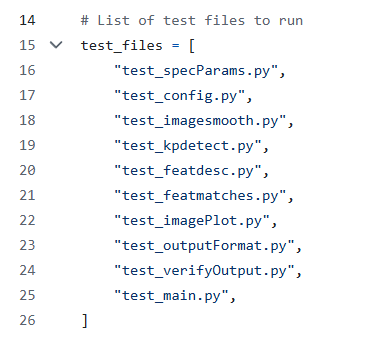
\includegraphics[width=0.5\linewidth]{images/unit_test_names.png}
  \caption{Outline of Automated Unit Tests}
  \label{unit_tests}
\end{figure}
		
\section{Trace to Requirements}
		
\section{Trace to Modules}		

\section{Code Coverage Metrics}

\bibliographystyle{plainnat}
\bibliography{../../refs/References}

\newpage{}
\section*{Appendix --- Reflection}

The information in this section will be used to evaluate the team members on the
graduate attribute of Reflection.

The purpose of reflection questions is to give you a chance to assess your own
learning and that of your group as a whole, and to find ways to improve in the
future. Reflection is an important part of the learning process.  Reflection is
also an essential component of a successful software development process.  

Reflections are most interesting and useful when they're honest, even if the
stories they tell are imperfect. You will be marked based on your depth of
thought and analysis, and not based on the content of the reflections
themselves. Thus, for full marks we encourage you to answer openly and honestly
and to avoid simply writing ``what you think the evaluator wants to hear.''

Please answer the following questions.  Some questions can be answered on the
team level, but where appropriate, each team member should write their own
response:


\begin{enumerate}
  \item What went well while writing this deliverable? 
  \item What pain points did you experience during this deliverable, and how
    did you resolve them?
  \item Which parts of this document stemmed from speaking to your client(s) or
  a proxy (e.g. your peers)? Which ones were not, and why?
  \item In what ways was the Verification and Validation (VnV) Plan different
  from the activities that were actually conducted for VnV?  If there were
  differences, what changes required the modification in the plan?  Why did
  these changes occur?  Would you be able to anticipate these changes in future
  projects?  If there weren't any differences, how was your team able to clearly
  predict a feasible amount of effort and the right tasks needed to build the
  evidence that demonstrates the required quality?  (It is expected that most
  teams will have had to deviate from their original VnV Plan.)
\end{enumerate}

\end{document}